%--------------------------------------------------------------
% tesi.tex 
%--------------------------------------------------------------
% Corso di Laurea in Informatica 
% http://if.dsi.unifi.it/
% @Facolt\`a di Scienze Matematiche, Fisiche e Naturali
% @Universit\`a degli Studi di Firenze
%--------------------------------------------------------------
% - template for the main file of Informatica@Unifi Thesis 
% - based on Classic Thesis Style Copyright (C) 2008 
%   Andr\'e Miede http://www.miede.de   
%--------------------------------------------------------------

\documentclass[twoside,openright,titlepage,fleqn,
,	headinclude,12pt,a4paper,BCOR5mm,footinclude,table]{scrbook}
%--------------------------------------------------------------
\newcommand{\myItalianTitle}{Gestione intelligente dei servizi in luoghi affollati\xspace}
\newcommand{\myEnglishTitle}{\textbf{E}vent\textbf{S} in crowd\textbf{E}d places: a sma\textbf{R}t ser\textbf{V}ice man\textbf{A}geme\textbf{NT}\xspace}
% use the right myDegree option
\newcommand{\myDegree}{Corso di Laurea in Informatica\xspace}
%\newcommand{\myDegree}{
	%Corso di Laurea Specialistica in Scienze e Tecnologie 
	%dell'Informazione\xspace}
\newcommand{\myName}{Yuri Bacciarini\xspace}
\newcommand{\myProf}{Rosario Pugliese\xspace}
\newcommand{\myOtherProf}{Nome Cognome\xspace}
\newcommand{\mySupervisor}{Nome Cognome\xspace}
\newcommand{\myFaculty}{
	Scuola di Scienze Matematiche, Fisiche e Naturali\xspace}
\newcommand{\myUni}{\protect{
	Universit\`a degli Studi di Firenze}\xspace}
\newcommand{\myLocation}{Firenze\xspace}
\newcommand{\myTime}{Anno Accademico 2018-2019\xspace}
\newcommand{\myVersion}{Version 0.1\xspace}
%--------------------------------------------------------------

\usepackage[italian]{babel}
\usepackage[utf8]{inputenc} 
\usepackage[T1]{fontenc} 
\usepackage[square,numbers]{natbib} 
\usepackage[fleqn]{amsmath}  
\usepackage{ellipsis}
\usepackage{listings}
\usepackage{subfig}
\usepackage{caption}
\usepackage{appendix}
\usepackage{siunitx}
\usepackage{url}
\usepackage{float}
\usepackage{multicol}
\usepackage{url}

%--------------------------------------------------------------
\usepackage{dia-classicthesis-ldpkg}
%--------------------------------------------------------------


%
% Options for classicthesis.sty:
% tocaligned eulerchapternumbers drafting linedheaders 
% listsseparated subfig nochapters beramono eulermath parts 
% minionpro pdfspacing
\usepackage[eulerchapternumbers,linedheaders,subfig,beramono,eulermath,
parts]{classicthesis}
%--------------------------------------------------------------
\newlength{\abcd} % for ab..z string length calculation
% how all the floats will be aligned
\newcommand{\myfloatalign}{\centering} 
\setlength{\extrarowheight}{3pt} % increase table row height
\captionsetup{format=hang,font=small}
%--------------------------------------------------------------
% Layout setting
%--------------------------------------------------------------
\usepackage{geometry}
\geometry{
	a4paper,
	ignoremp,
	bindingoffset = 1cm, 
	textwidth     = 13.5cm,
	textheight    = 21.5cm,
	lmargin       = 3.5cm, % left margin
	tmargin       = 4cm    % top margin 
}




%%
%% Julia definition (c) 2014 Jubobs
%%
\lstdefinelanguage{Julia}%
  {morekeywords={abstract,break,case,catch,const,continue,do,else,elseif,%
      end,export,false,for,function,immutable,import,importall,if,in,%
      macro,module,otherwise,quote,return,switch,true,try,type,typealias,%
      using,while},%
   sensitive=true,%
   alsoother={},%
   morecomment=[l]\#,%
   morecomment=[n]{\#=}{=\#},%
   morestring=[s]{"}{"},%
   morestring=[m]{'}{'},%
}[keywords,comments,strings]%

\lstset{%
    language         = Julia,
    basicstyle       = \ttfamily,
    keywordstyle     = \bfseries\color{blue},
    stringstyle      = \color{magenta},
    commentstyle     = \color{ForestGreen},
    showstringspaces = false,
}
%%%

\usepackage{tikz}
\usetikzlibrary{arrows}
\usetikzlibrary{positioning}
\tikzset{main node/.style={circle,fill=blue!20,draw,minimum size=1cm,inner sep=0pt},
            }



%--------------------------------------------------------------
\begin{document}
\frenchspacing
\raggedbottom
\pagenumbering{roman}
\pagestyle{plain}
%--------------------------------------------------------------
% Frontmatter
%--------------------------------------------------------------


%--------------------------------------------------------------
% titlepage.tex (use thesis.tex as main file)
%--------------------------------------------------------------
\begin{titlepage}
	\begin{center}
   	\large
      \hfill
      \vfill
      \begingroup
         \includegraphics[scale=0.15]{img/logo}\\
%			\spacedallcaps{\myUni} \\ 
			\myFaculty \\
			\myDegree \\ 
			\vspace{0.5cm}
         \vspace{0.5cm}    
           
      \endgroup 
      \vfill 
      \begingroup
      	\color{Maroon}\spacedallcaps{\myItalianTitle} \\ $\ $\\
      	\spacedallcaps{\myEnglishTitle} \\ 	
	\bigskip
      \endgroup
      \spacedlowsmallcaps{\myName} \\ $\ $\\
      \spacedlowsmallcaps{\myProf}
      \vfill 
      \vfill
    
      \vfill
      \vfill
      \myTime
      \vfill                      
	\end{center}        
\end{titlepage}   
%--------------------------------------------------------------
% back titlepage
%--------------------------------------------------------------
   \newpage
	\thispagestyle{empty}
	\hfill
	\vfill
	\noindent\myName: 
	\textit{\myItalianTitle,} 
	\myDegree, \textcopyright\ \myTime
%--------------------------------------------------------------
% back titlepage end
%--------------------------------------------------------------

\pagestyle{scrheadings}
%--------------------------------------------------------------
% Mainmatter
%--------------------------------------------------------------
\pagenumbering{arabic}
% use \cleardoublepage here to avoid problems with pdfbookmark
%\include{intro} % use \myChapter command instead of \chapter
%\cleardoublepage\myPart{Part I}
%\include{chapter01}
%\cleardoublepage\myPart{Part II}
%\include{chapter02}
%\include{chapter03}
\tableofcontents
%\listoftables
%\listoffigures
\chapter{eServant}

\section{Panoramica}
eServant [1] è un progetto di ricerca cofinanziato con fondi POR-CReO FESR 2014 - 2020 - Bandi per aiuti agli investimenti in ricerca, sviluppo e innovazione RSI. QUID Informatica S.p.A è Capofila di un raggruppamento di Aziende ed Organismi di ricerca finalizzato alla realizzazione del progetto.
\paragraph{}

Il focus del progetto è la gestione innovativa dei processi collegati ai grandi eventi (musicali, sportivi, del tempo libero o del lavoro) che hanno luogo all’interno di impianti e strutture, sia in termini di comunicazione e controllo, sia in termini di servizi innovativi per gli spettatori/utenti, andando a disegnare un progetto di impianto intelligente, inserito all’interno di una struttura di città intelligente, costruita per un cittadino consapevole, che valorizzi i temi della responsabilità sociale e civile e  della sostenibilità.
\paragraph{}

Si tratta quindi di un insieme di processi, che sono gestiti in modo assolutamente innovativo, sino a creare un processo evoluto, costituito dalla piattaforma eServant, che viene industrializzato in una struttura hardware e software altamente replicabile.
\paragraph{}

L’obiettivo operativo è quindi quello di progettare un modello di centro-servizi per la produzione, il controllo e la distribuzione di contenuti all’interno di grandi impianti, sportivi e non, in occasione di eventi specifici come mostrato nella Figura 1.
\paragraph{}

Il concetto di impianto al quale presta i suoi servizi il progetto eServant è molto ampio.
Ci sono nel settore dello sport in Italia circa 150.000 impianti sportivi, di tutte le taglie. Ci sono gli impianti per il teatro (1.162), i centri commerciali, retail park e factory outlet (956), migliaia di punti vendita della GDO, oltre 200 parchi nella sola Toscana, i comuni con decine di migliaia tra centri storici, aree monumentali, aree archeologiche, complessi monumentali e luoghi della cultura, oltre 57.000 plessi scolastici ed un numero incalcolabile di luoghi ove si esprime la socialità [2].
Non però una socialità «generalistica» ed indistinta, come nei social tradizionali tipo Facebook (dove si parla di tutto e di nulla), ma bensì una socialità caratterizzata da tre fattori unici e comuni:
tante persone
raccolte in un unico spazio
all’interno del quale condividono un comune interesse.
È questo un tipo di contesto non esplorato, al quale il progetto eServant prova a dare delle risposte e dei servizi mirati.
\paragraph{}

La sperimentazione del progetto eServant si è svolta presso l’impianto universitario PIN a Prato nel mese di Dicembre 2018.
\paragraph{}

\begin{figure}[h!]
    \centering  
    \caption{eServant flow}
    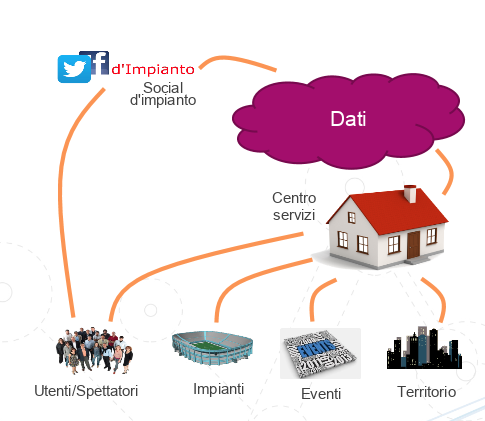
\includegraphics[scale=0.8]{img/cap1/eservant}
\end{figure}

\paragraph{}

\section{Aziende coinvolte}

\textbf{Quid Informatica spa}\\
Come capofila di progetto, Quid Informatica spa si è occupata di sviluppare e mettere a disposizione l’infrastruttura tecnologica per fruire i moduli sviluppati dai vari partner.
\\\\
\textbf{Sokom srl}\\
Sokom srl si è occupata dei cablaggi e della disposizione dei vari access point necessari per fare comunicare i dispositivi IoT posti all’interno dell’impianto.
\\\\
\textbf{Magenta srl}\\
Magenta srl si è occupata dei sensori IoT per il conteggio delle persone tramite hardware Raspberry ed in parallelo al recupero di dati da fonti open source, come Lamma e Open Toscana.
\\\\
\textbf{MICC}\\
Il MICC invece si è occupato dell’ottenimento della densità di persone in alcuni punti strategici dell’impianto di sperimentazione. Ha inoltre sviluppato un modulo di mappe, il quale, insieme alla tecnologia precedente, permette di consigliare ai partecipanti eventuali percorsi alternativi in caso di affollamento.
Infine, il MICC ha ideato anche un motore di affinità tra visitatori grazie al collegamento social degli stessi.
\\\\
\textbf{DIISM}\\
Il dipartimento Ingegneria dell’informazione e Scienze Matematiche di Siena è fornitore e configuratore dei dispositivi iBeacon che tramite la tecnologia BLE (bluetooth low energy) ci ha permesso di ottenere la posizione delle persone all’interno dell’impianto di sperimentazione anche in assenza di GPS.
\paragraph{}

\section{Casi d'uso}

\begin{figure}[h!]
    \centering  
    \caption{Casi d'uso eServant}
    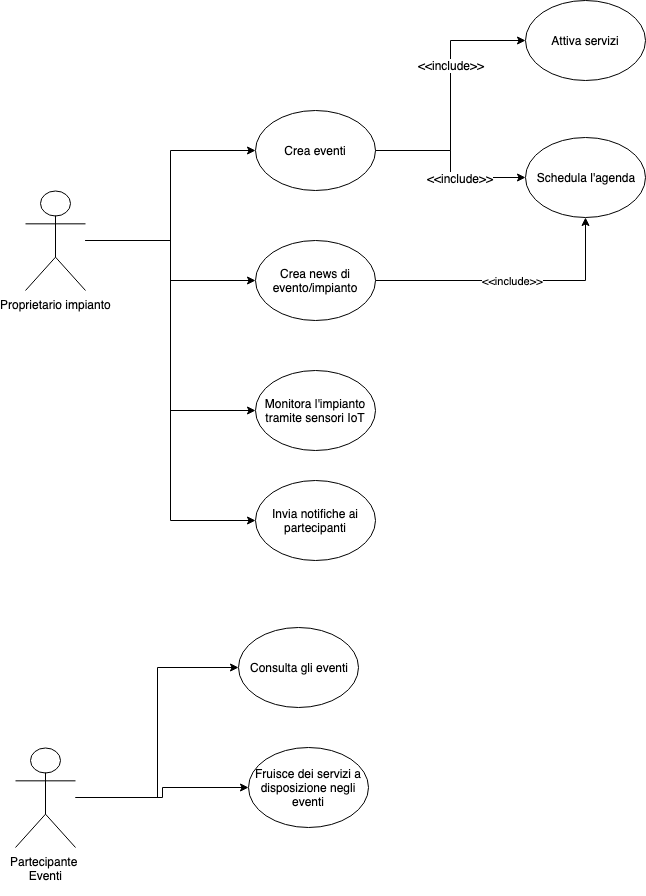
\includegraphics[scale=0.5]{img/cap1/casidiuso}
\end{figure}
La figura 2 descrive le funzioni e servizi offerti dal progetto eServant e percepiti dagli attori che interagiscono col sistema stesso [3].
\\\\\\\\Gli attori coinvolti nelle funzioni di eServant sono due:
\begin{itemize}
    \item proprietario impianto;
    \item partecipante eventi;
\end{itemize}

Il proprietario dell'impianto gestisce gli eventi nella propria struttura, potendo nello specifico attivare servizi specifici e schedularne l'agenda.
Come vediamo dalla figura 2 la funzione per schedulare l'agenda è inclusa anche nella creazione delle news riguardanti l'evento specifico o a
carattere generico dell'impianto.
Infine il proprietario dell'impianto può monitorare la propria struttura grazie a sensori IoT e mettersi in cotatto con i partecipanti tramite notifiche push.

L'attore "Partecipante Eventi" invece, fruisce di tutti quei servizi configurati dal gestore dell'impianto; può quindi consultare gli eventi disponibili ed
i relativi dettagli.

\section{Back-end}
OSGI (Open Service Gateway Initiative)[4] è  è una specifica che permette di costruire
applicazioni modulari a componenti (detti “bundle”) e che introduce una
programmazione Service Oriented, permettendo una separazione tra interfaccia ed
implementazione molto più rigorosa di quella nativa Java.
Il nucleo delle specifiche è un framework che definisce la gestione del modello del ciclo di vita del software, i moduli (chiamati bundle), un service registry e un ambiente di esecuzione. 
L’aumento della complessità in un prodotto software, sia esso embedded, client o server, richiede codice modulare ma anche sistemi che siano estensibili dinamicamente, molto più in applicazioni tipo quelle di eSERVANT. Il framework OSGI implementa un modello a componenti completo e dinamico cioè quello che manca all’ambiente Java. 
OSGi risolve molti dei problemi legati allo scarso supporto di Java nella modularità e nel dinamismo ed in tal senso OSGI è un framework che permette di fornire: 
\begin{itemize}
\item un sistema modulare per la piattaforma Java;
\item un sistema dinamico, che consente l’installazione, l’avvio, lo stop e la
rimozione dei moduli a runtime, senza quindi necessitare di riavvii;
\item un sistema orientato ai servizi, i quali possono essere dinamicamente
registrati ed utilizzati nella macchina virtuale Java;
\end{itemize}




Per tutti i motivi indicati OSGI viene adottato all’interno dell’architettura di eSERVANT,
come strumento per lo sviluppo delle applicazioni di backend di tutti i partner del
progetto.

\subsection{Microservizi}

\begin{figure}[h!]
    \centering  
    \caption{Architettura}
    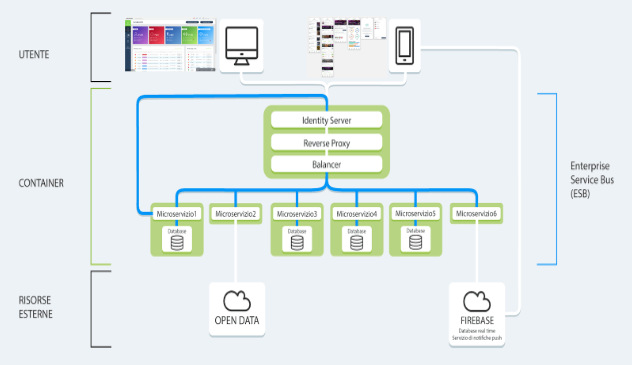
\includegraphics[scale=0.5]{img/cap1/architecture}
\end{figure}

Dalla figura 3 vediamo qual'è il flusso di una richiesta proveniente dall'utente fruitore del backoffice web o
dell'applicazione mobile.
Tutte le richieste HTTPS vengono intercettate prima di tutto dall'identity server che verifica tramite JWT token
se l'utente è autorizzato a ottenere le risorse richieste.
Successivamente, le richieste vengono smistate al corretto microservizio specializzato grazie al reverse proxy.
Visto che i microservizi sono progettati per avere più repliche, il balancer permette di astrarle e bilanciare correttamente
il carico di lavoro.

Ogni microservizio, come da figura 3, se necessario ha internamente un proprio database
che nessun'altro oltre a lui può accederci.

L'ultima parte, quella delle risorse esterne, rappresenta tutti servizi fuori dalla rete
dei microservizi; "open data" per esempio sono API pubbliche per il recupero di dati pubblici (es. Lamma per il meteo)
mentre "Firebase" sono una serie di servizi cloud per push notification e real time database [5].

\subsection{Swagger (API)}
Swagger [6] è un insieme di specifiche e di strumenti che mirano a semplificare e
standardizzare i processi di documentazione di API per servizi web RESTful, il tutto su
di una piattaforma di tipo open-source.
Il cuore di Swagger consiste in un file testuale (in formato sia YAML che JSON) dove
sono descritte tutte le funzionalità di un’applicazione web e i dettagli di input e output
in un formato studiato per essere interpretabile correttamente sia dagli umani che
dalle macchine.
\paragraph{}

I vantaggi di questa standardizzazione sono molti, come una migliore e più condivisibile
esplorazione delle funzionalità di un’applicazione, oltre che alla possibilità di
generare codice client/server sfruttando direttamente i vincoli definiti nello schema. Infatti, i metadati presenti nel file forniscono informazioni sufficienti sia per
generare il componente backend con le rotte http e la validazione degli input, sia la parte client che in modo automatico può adattarsi all’evoluzione delle API del backend. La generazione della parte server è sicuramente vantaggiosa in quanto è possibile concentrarsi direttamente sulla programmazione della logica di business, senza doversi preoccupare di come questa va ad interagire con il sistema al quale si interfaccia. Swagger è sostanzialmente composto da tre moduli: 
\begin{enumerate}
    \item Swagger Editor: è lo strumento per iniziare rapidamente nell’attività di
    progettazione di una nuova API o per la sua modifica in un potente editor che
    visualizza visivamente la definizione Swagger e fornisce feedback in tempo
    reale;
    \item Swagger Codegen: è lo strumento che crea ed abilitata le varie applicazioni al
    consumo delle API utilizzabili su una molteplicità di linguaggi di sviluppo (Java,
    Javascript Perl, PHP, Python, Ruby, Scala;
    \item Swagger UI: è lo strumento che permette con un tool visuale il
    consumo delle API da parte delle varie applicazioni;
\end{enumerate}


\paragraph{}

Per tutti i motivi indicati Swagger viene adottato all’interno dell’architettura di
eSERVANT, come strumento per lo sviluppo delle varie API di interfacciamento verso
la applicazioni dei partner.


\subsection{Database (relazionale + documentale)}
I due tipi di database usati nel progetto sono stati PostgreSQL e MongoDB, il primo relazionale e il secondo orientato a documenti.
\paragraph{}

PostgreSQL [7] è noto come il più avanzato sistema di gestione di dati open-source
disponibile sul mercato.
Si tratta di un DBMS (DataBase Management System), ossia di un vero e proprio insieme di componenti software in grado di permettere la creazione e la manipolazione di un database.
\paragraph{}

Ma PostgreSQL è anche un ORDBMS (Object Relational DataBase Management System), ossia un sistema che supporta un modello di database object oriented, che implementa oggetti, classi, ereditarietà e permette l’estensione del modello di dati con tipi di dati e metodi
personalizzati.
È altamente portatile, infatti è disponibile praticamente su tutte le distribuzioni di Linux, Unix, Windows, Mac OS, ecc.
\paragraph{}

Per tutti i motivi indicati PostgreSQL viene adottato all’interno dell’architettura di eSERVANT come il database di riferimento, utilizzato da tutte le applicazioni che necessitano del supporto di un database di tipo relazionale.
Tutta la gestione massiva dei dati viene invece gestita attraverso il database non-SQL
MongoDB.

\paragraph{}
MongoDB [8], invece, è un DBMS orientato alla gestione dei testi che ha come obiettivo quello di strutturare delle basi di dati testuali, in particolare con dati poco strutturati.
Questo DBMS eredita il meccanismo di storage dal paradigma doc-oriented che consiste nel memorizzare ogni record come documento che non possiede caratteristiche predeterminate.
Nei DB orientati ai documenti, si segue una metodologia differente rispetto al modello relazionale: si accorpano quanto più possibile gli oggetti, creando delle macro entità dal massimo contenuto informativo. Questi oggetti incorporano tutte le notizie di cui necessitano per una determinata semantica.
Pertanto MongoDB non possiede uno schema e ogni documento non è strutturato, ha solo due chiavi obbligatorie:
id, che serve per identificare univocamente il documento (è comparabile, semanticamente, alla chiave primaria dei database relazionali)
e rev, che viene utilizzata per la gestione delle revisioni (ad ogni operazione di modifica infatti la chiave rev viene aggiornata).
\paragraph{}

Pertanto si può interrogare il DBMS anche per versioni del documento non recenti perché mantiene in memoria tutte le versioni.
MongoDB gestisce anche la ridondanza dei dati per rimediare a malfunzionamenti.
\paragraph{}

Per evitare che lo sviluppatore acceda direttamente al database tramite linguaggio sql per PostgreSQL o tramite i metodi specifici per MongoDB,
entra in gioco il framework Hibernate.

Hibernate [9] (talvolta abbreviato in H8) è una piattaforma middleware open source per lo sviluppo di applicazioni Java che fornisce un servizio di Object-relational mapping (ORM), ovvero che gestisce la rappresentazione e il mantenimento su database relazionale di un sistema di oggetti Java. Lo scopo principale di Hibernate è quello di fornire un mapping delle
classi Java in tabelle di un database relazionale; sulla base di questo
mapping Hibernate gestisce il salvataggio degli oggetti di tali classi su database. Si occupa inoltre del reperimento degli oggetti da database, producendo ed eseguendo automaticamente le query SQL necessarie al recupero delle informazioni e la successiva reistanziazione dell’oggetto precedentemente “ibernato” (mappato su database).
Hibernate in pratica esonera lo sviluppatore dal lavoro inerente la persistenza dei dati.
Fortunatamente Hibernate gestisce una persistenza trasparente per “Plain Old Java
Object”.


\section{Front-end}


Lo sviluppo lato app è stato implementato usando il framework di sviluppo applicazioni mobile ibride Ionic.
Questo framework utilizza di default l’engine Angular ed aggiunge ad esso una serie di funzioni “speciali” che permettono l’accesso a routine native, es. accensione camera dispositivo. Le funzioni “speciali” sono realizzate dalla libreria Cordova che implementa il ponte tra Javascript e il codice nativo Android/IOS.
\paragraph{}

Il punto di forza di Ionic è l’essere un framework ibrido. Scrivendo quindi un unico progetto in Javascript è possibile eseguirlo immediatamente su 3 piattaforme diverse: web, Android e IOS.
\paragraph{}

Angular 2 è un framework Javascript pensato per lo sviluppo di applicazioni di tipo web, sia per mobile che per desktop, basato sul progetto open-source prima di Angular JS e poi di Angular.
\paragraph{}

Angular da un lato esalta e potenzia l’approccio dichiarativo di HTML nella definizione
dell’interfaccia grafica, dall’altro fornisce strumenti per la costruzione di un’architettura modulare e testabile della logica applicativa di un’applicazione.
In questo senso Angular fornisce tutto quanto occorre per creare applicazioni moderne che
sfruttano le più recenti tecnologie, come ad esempio le Single Page Application, cioè
applicazioni le cui risorse vengono caricate dinamicamente su richiesta, senza necessità di
ricaricare l’intera pagina, cosa particolarmente utile in una applicazione del tipo eSERVANT.
\paragraph{}

Le caratteristiche di Angular 2 sono [10]:

\begin{itemize}
    \item  \textbf{mobile first}: uno degli obiettivi del nuovo Angular è di proporsi per lo
    sviluppo di applicazioni Web sia per l’ambiente desktop che per il mobile.
    Infatti, Angular 2 supporta di default eventi touch e gesture e promette
    elevate prestazioni per assicurare una interazione fluida sui dispositivi
    mobile;
    \item \textbf{riduzione della curva di apprendimento}: Angular 2 ha ottimizzato e
    semplificato di molto le complessità insite nella realizzazione di interfacce
    sia per mobile che per desktop;
    \item \textbf{modultarità}: l’architettura di Angular 2 è altamente modulare e favorisce la
    scrittura di applicazioni modulari e la maggior parte dei componenti del
    framework è opzionale ed è possibile sostituirli con altri di terze parti o
    sviluppati in proprio;
    \item \textbf{prestazioni}: un’attenzione particolare è stata posta sulle prestazioni del
    framework e sulla riduzione dei tempi di caricamento e boostrapping delle
    applicazioni;
\end{itemize}

Per tutti i motivi indicati Angular 2 viene adottato all’interno dell’architettura di
eSERVANT, come strumento per il progetto delle interfacce sia su mobile (e quindi per
gli utenti/spettatori) che su desktop (e quindi dedicate alla centrale di controllo e
gestione).

\chapter{Applicazione mobile}
Empty thesis model

\section{Funzionalita'}
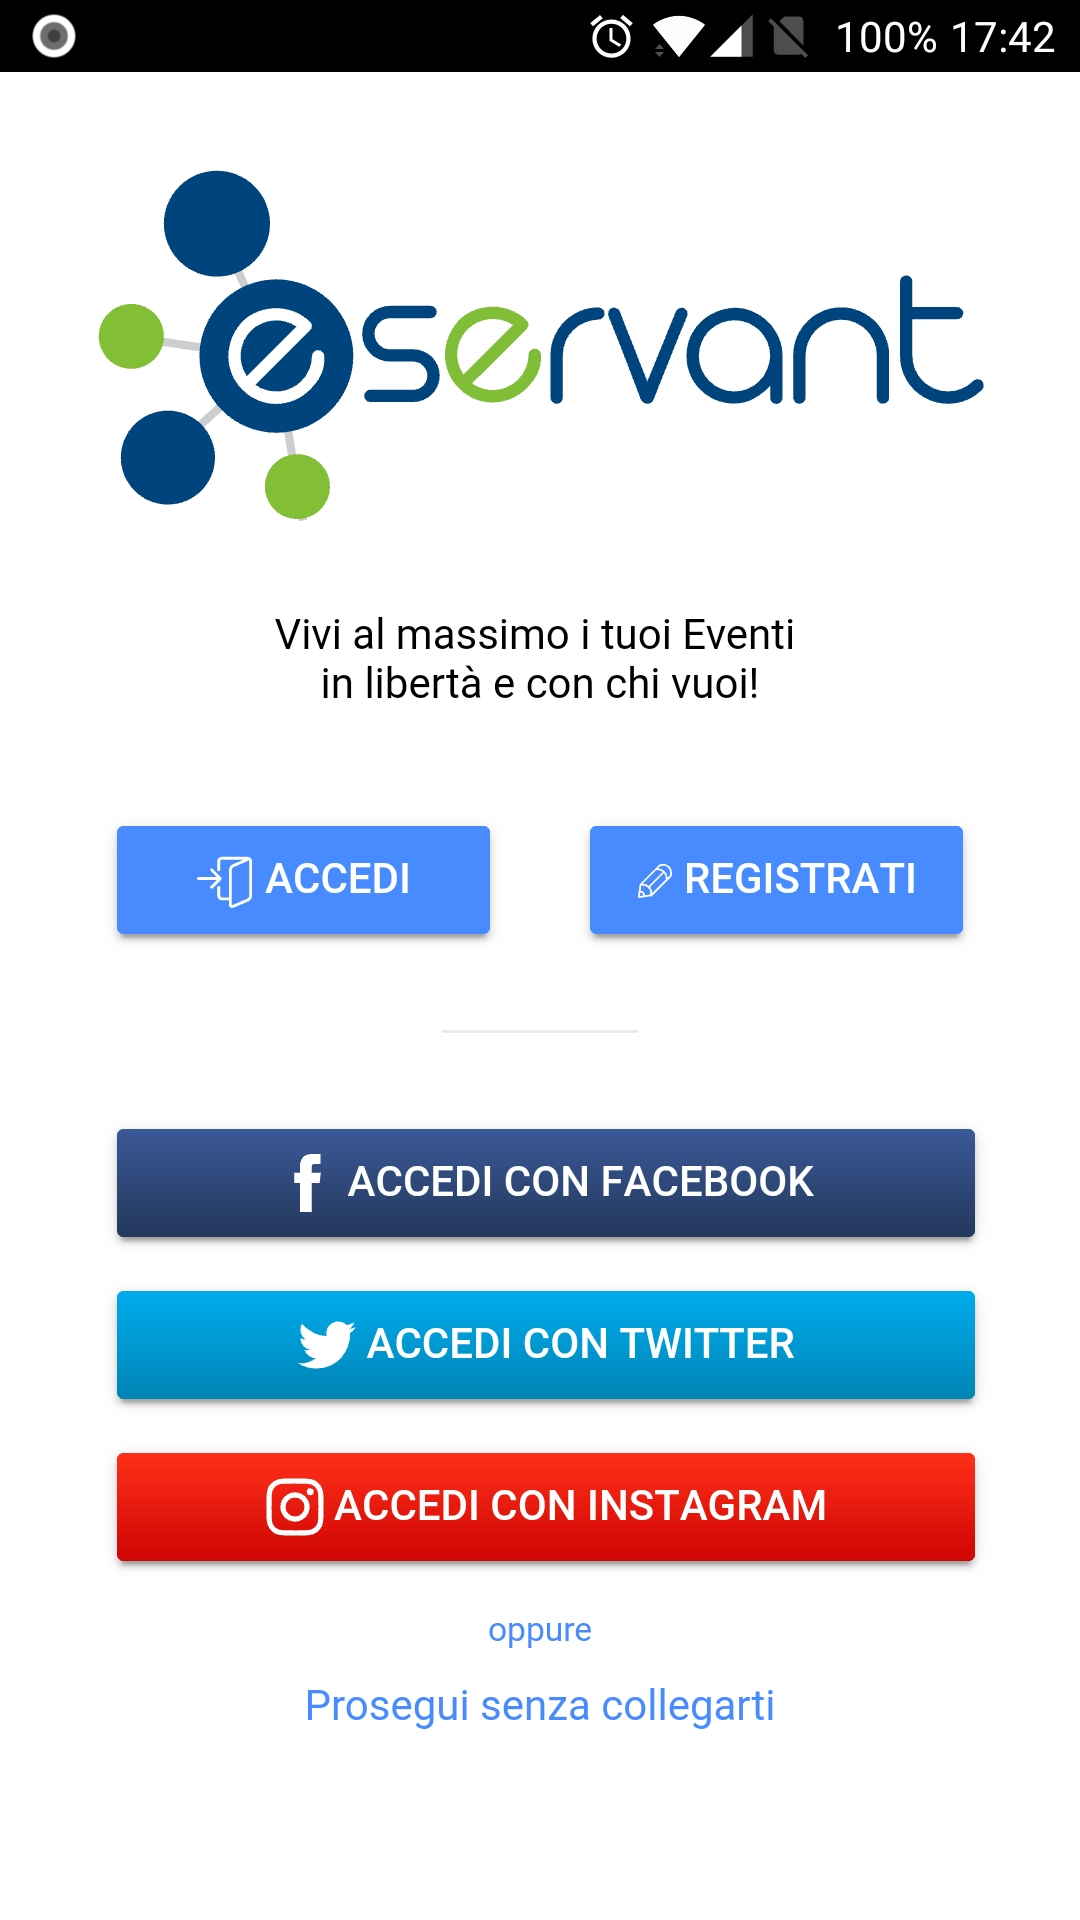
\includegraphics[scale=0.15]{img/cap2/1}\\

\includegraphics[scale=0.15]{img/cap2/2}\\

\section{Framework Ionic}
\subsection{NgRx gestore stato}
\subsection{Android}
\subsection{IOS}
\section{Geolocalizzazione}
\subsection{iBeacon}
\subsection{QRcode}
\subsection{GPS}
\section{Navigazione (mappe intelligenti)}
\section{Chatbot (DialogFlow)}

\chapter{Backoffice}
Il Backoffice è l'applicazione web che permette ai gestori degli impianti presenti su eServant di:
\begin{itemize}
    \item configurare i propri impianti, per ogni impianto gli eventi e per ogni evento i servizi disponibili;
    \item monitorare real-time l'impianto analizzando i dati provenienti dai sensori IoT;
    \item monitorare e analizzare offline le prestazioni del sistema/impianto dopo un evento o in un certo periodo.
\end{itemize}
Vediamo nello screenshot della dashboard in Figura 19 le funzioni di monitoraggio dell'impianto.
\begin{figure}[H]
    \centering  
    \caption{Screenshot dashboard}
    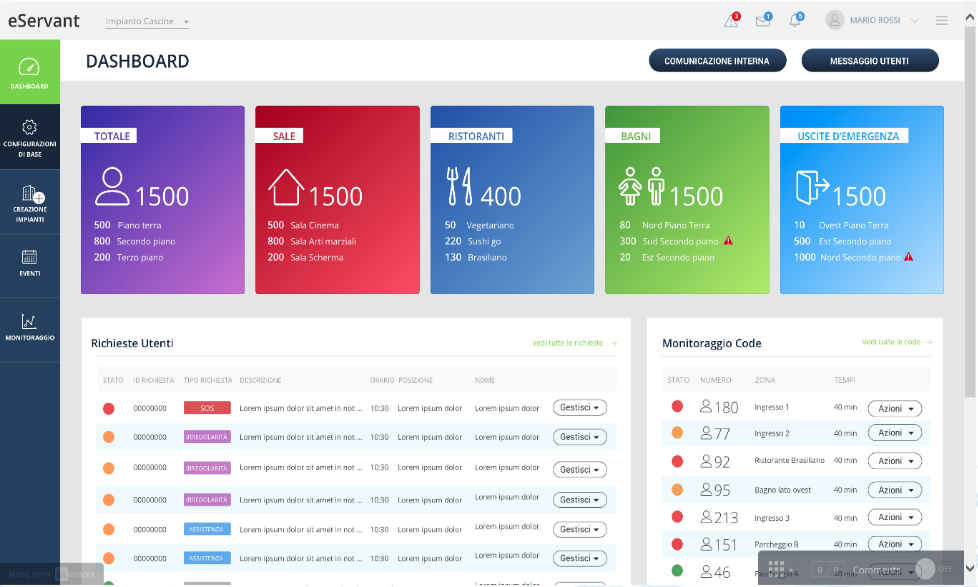
\includegraphics[scale=0.4]{img/cap3/backoffice}
\end{figure}

Il backoffice di eServant è stato realizzato con il framework Angular usando interamente Material Design come
sistema di progettazione dell'esperienza utente.
Material Design è un framework open source dell'azienda Google che aiuta i team a creare esperienze digitali
di alta qualità in breve tempo.

\section{Material Design}
Material Design [31] mette a disposizione al team di sviluppo un set di componenti plugAndPlay solo da personalizzare
secondo il tema del brand utilizzatore.
Il principale vantaggio riscontrato è stata la velocità di sviluppo. Avendo nella maggior parte dei
casi dei componenti pronti all'uso, ci ha permesso di concentrarci sulla logica in Typescript invece che
sull'esperienza utente (non da sottovalutare).

I principali componenti messi a disposizione da Material Design di Google in Angular [32] sono:

\begin{itemize}
    \item Componenti per i form;
    \item Navigazione;
    \item Layout;
    \item Bottoni;
    \item Popup;
    \item Tabelle dati.
\end{itemize}

Riportiamo un frammento di codice HTML usato nel backoffice di eServant ed il relativo effetto
nell'interfaccia utente nella Figura 20.

\begin{lstlisting}[language=html]
<form class="newsform">
..
  <mat-form-field class="newsform__field">
    <input matInput placeholder="Titolo"">
  </mat-form-field>
..
</form>
\end{lstlisting}

\begin{figure}[H]
    \centering  
    \caption{Form creazione nuova news}
    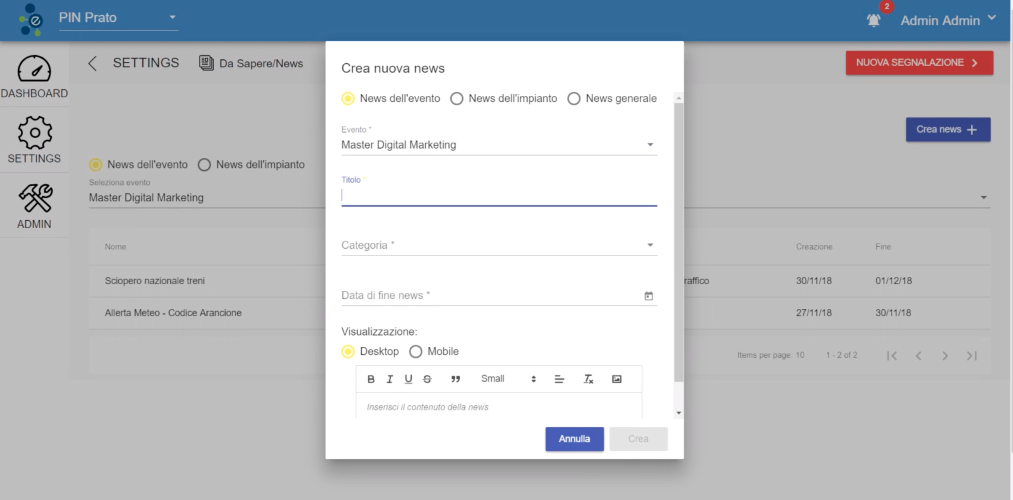
\includegraphics[scale=0.4]{img/cap3/backoffice-form}
\end{figure}

\section{BEM}
È noto che un'organizzazione corretta dei fogli di stile può aumentare significativamente la velocità
di sviluppo, il debug e l'implementazione di nuove feature. Purtroppo, molti codici CSS vengono
sviluppati senza alcuna convenzione di struttura o di nome. Ciò porta a una base di codice CSS 
non mantenibile a lungo termine.
Ecco una citazione molto importante dove si afferma che ci sono due principali problemi nell'informatica: l'invalidazione della cache e le convenzioni sui nomi.\\\\
"There are only two hard problems in Computer Science: cache invalidation and naming things" cit. Phil Karlton [33]\\

L'approccio BEM cerca di garantire a tutti i partecipanti attuali e futuri allo sviluppo di un sito web
lavorino con un singolo base code e parlino la stessa lingua. 

BEM [34] è l'acronimo di 
\begin{itemize}
\item Block;
\item Element;
\item Modifier.
\end{itemize}

\begin{figure}[H]
    \centering  
    \caption{Esempio di adozione BEM [35]}
    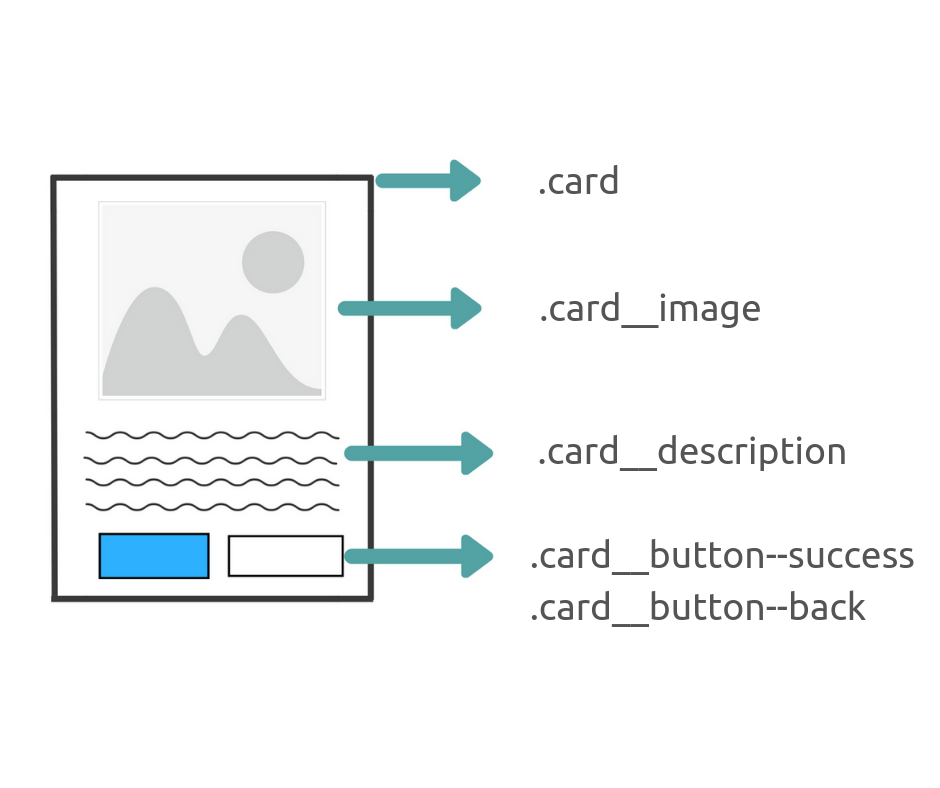
\includegraphics[scale=0.5]{img/cap3/bem-1}
\end{figure}

Analizziamo le classi CSS usate in Figura 21:

\begin{itemize}
    \item \textit{.card} è un \textbf{block};
    \item \textit{.card{\_}image} e  \textit{.card{\_}descriptor} sono \textbf{Element} di \textit{.card};
    \item \textit{.card{\_}image--success} e  \textit{.card{\_}descriptor--back} sono 
    \textbf{Modifier} di \textit{.card{\_}image}.
\end{itemize}

Vediamo come è stato usato BEM nel caso specifico dell'header rappresentato in Figura 22.

\begin{figure}[H]
    \centering  
    \caption{Header}
    
\includegraphics[scale=0.4]{img/cap3/header}
\end{figure}

\begin{lstlisting}[language=html]
<mat-toolbar class="header">
    <mat-toolbar-row>
        <img class="header__logo">
        <mat-select class="header__facilities">
            <mat-option *ngFor="let facility of facilities" [value]="facility.value">
            {{facility.display}}
            </mat-option>
        </mat-select>
        <mat-icon>alert</mat-icon>
        <div class="settings">
            <span class="settings__user">Admin</span>
            <mat-icon class="settings__icon settings__icon--closed">arrow-down</mat-icon>
        </div>
    </mat-toolbar-row>
</mat-toolbar>
\end{lstlisting}

\chapter{IoT}
Il progetto eServant include al suo interno due principali tecnologie che rientrano nella categoria
"Internet Of Things":
\begin{itemize}
    \item dispositivi BLE per geolocalizzare i partecipanti dove il GPS ha dei grandi limiti
    \item conta persone per monitorare il flusso nelle aule
\end{itemize}


Scendendo nel dettaglio, l'impianto PIN di Prato è stato attrezzato con una serie di dispositivi BLE 
(Bluetooth Low Energy) per intercettare i dispositivi mobili dei partecipanti e con un conta persone
situato all'ingresso della biblioteca.

\section{Bluetooth Low Energy}
I dispositivi BLE possono operare in modalità attiva o in modalità passiva, rispettivamente esistono
le seguenti due modalità:
\begin{itemize}
    \item ranging;
    \item advertising;
\end{itemize}


\subsection{Gateway}
I Gateway posizionati negli ingressi principali sono stati realizzati tramite single board computer 
Raspberry e rivestiti tramite case fissato a muro come in figura 23.
\begin{figure}[H]
    \caption{Dispositivo Gateway}
    \centering  
    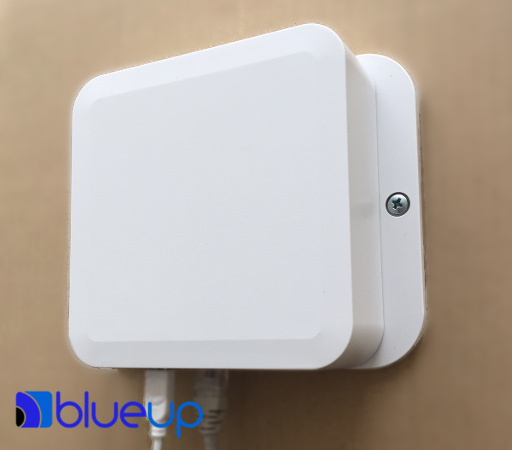
\includegraphics[scale=0.4]{img/cap4/gateway}
\end{figure}

Le principali componenti usate sono:
\begin{itemize}
    \item scheda di rete wireless;
    \item chip Bluetooth versione 5;
    \item PoE (Power over Ethernet);
\end{itemize}

I gateway forniti dall'azienda BlueUp hanno al loro interno già un firmware che all'avvio del sistema operativo
raspbian avvia il servizio di ranging.
La feature che distingue questi gateway è che sono programmati per chiamare un servizio HTTP custom 
al quale, tramite metodo POST, vengono inviati la lista degli ibeacon in modalità advertising intercettati.

Queste chiamate HTTP, ricevute da un microservizio specializzato di eServant, registrano che nella data
di ricezione sono stati intercettati una serie di ibeacon con una determinata prossimità (BASSA,MEDIA,ALTA).

Visto che i gateway hanno una posizione fissa all'interno dell'impianto, sono stati catalogati nel nostro
database con le coordinate di installazione.
Queste coordinate rappresenteranno la posizione dei dispositivi mobili (in modalità advertising) quando quest'ultimi
vengono intercettati dal gateway attivo.

\subsection{iBeacon passivi}
Gli iBeacon passivi sono un'altro dispositivo standalone dotati di batteria e facilmente maneggevoli per
geolocalizzare un dispositivo all'interno di uno spazio indoor.
Rispetto ai gateway attivi hanno il vantaggio di essere molto più economici (5 volte meno) e di essere
dotati di batterie al litio.

Gli smartphone con eServant installata (in modalità attiva o in background), potranno intercettare
questi dispositivi (come in figura 24) ed inviare tramite HTTP al microservizio specializzato l'ID dell'ibeacon rilevato
per permettere di geolocalizzare il partecipante nelle coordinate dell'ibeacon storicizzate nel nostro
database.

\begin{figure}[H]
    \centering  
    \caption{iBeacon passivi in azione}
    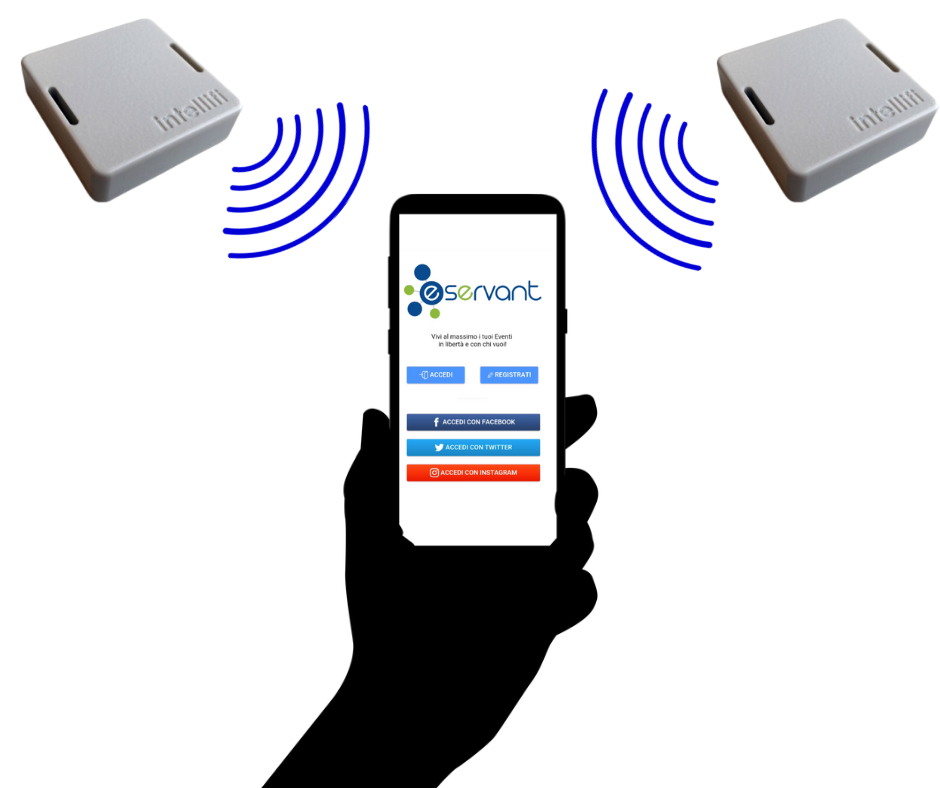
\includegraphics[scale=0.4]{img/cap4/ibeacon-advertising}
\end{figure}

\subsection{iBeacon Wearable}
\begin{figure}[H]
    \centering  
    \caption{iBeacon indossabile}
    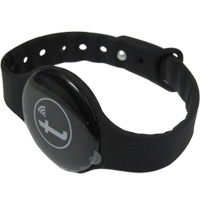
\includegraphics[scale=0.4]{img/cap4/wearable}
\end{figure}
I braccialetti BLE svolgono l'esatto compito degli iBeacon passivi sopra descritti ma vengono utilizzati
con una strategia diversa all'interno di eServant.
Il caso d'uso principale è permettere ai genitori di monitorare real-time la posizione dei propri
figli all'interno di un impianto affollato.
Al genitore, all'ingresso dell'impianto, verranno consegnati un braccialetto (come in figura 25) per ogni figlio.

Nella sezione ricerca un minore dell'app eServant scansionerà il QRcode sopra il braccialetto e da quel momento
in poi il suo utente sarà abilitato a monitorare l'ultima posizione rilevata di ogni singolo braccialetto.
L'assegnazione dei braccialetti viene rilasciata in maniera spontanea all'uscita dall'impianto oppure 
tramite un sistema automatico alcune ore dopo la fine dell'evento (nel caso in cui il genitore non riconsegni
i braccialetti).

I passi sopra descritti sono riportati in figura 26.
\begin{figure}[htp]
    \centering  
    \caption{Caso d'uso braccialetti iBeacon}
    \subfloat[Scanner]{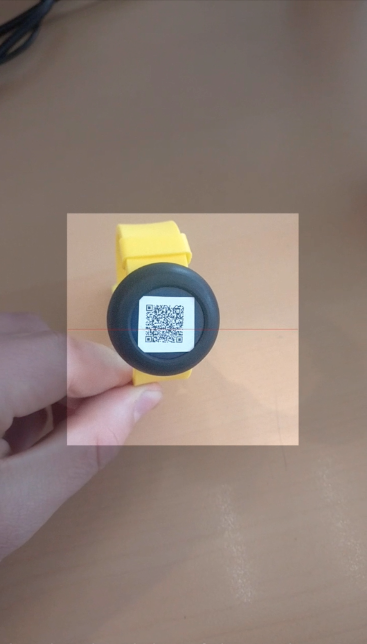
\includegraphics[scale=0.3]{img/cap4/wearable-1}}
    \subfloat[Nome]{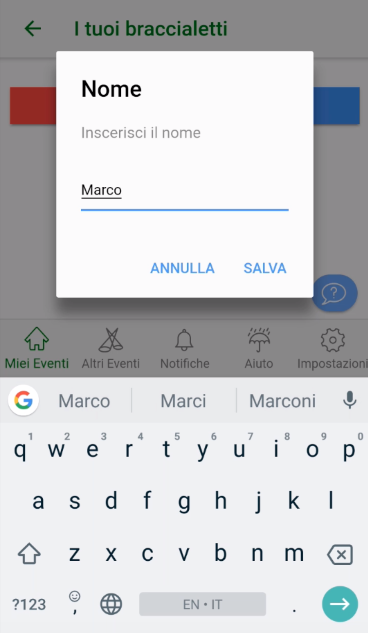
\includegraphics[scale=0.3]{img/cap4/wearable-2}}
    \subfloat[Braccialetti registrati]{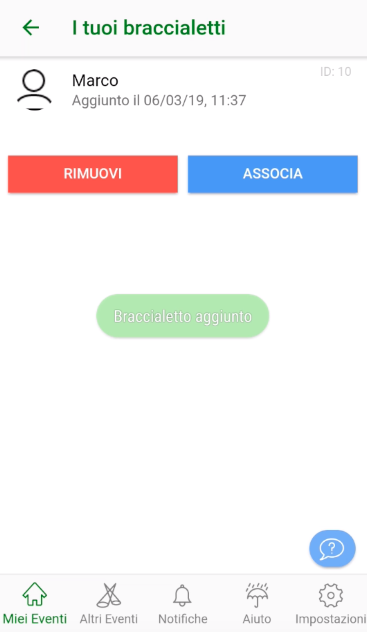
\includegraphics[scale=0.3]{img/cap4/wearable-3}}
    \subfloat[Geolocalizzazione]{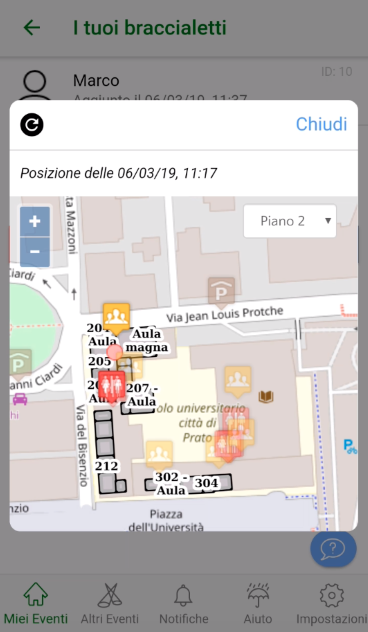
\includegraphics[scale=0.3]{img/cap4/wearable-4}}

\end{figure}

\subsection{Smartphone}
Gli smarthone dei partecipanti agli eventi, tramite l'app di eServant attiva o in background, agiscono
sia in modalità advertising per essere intercettati da eventuali gateway sia in modalità attiva (scanning) per 
intercettare i dispositivi passivi.

\section{Conta persone}

\begin{figure}[H]
    \centering  
    \caption{Single board computer Raspberry}
    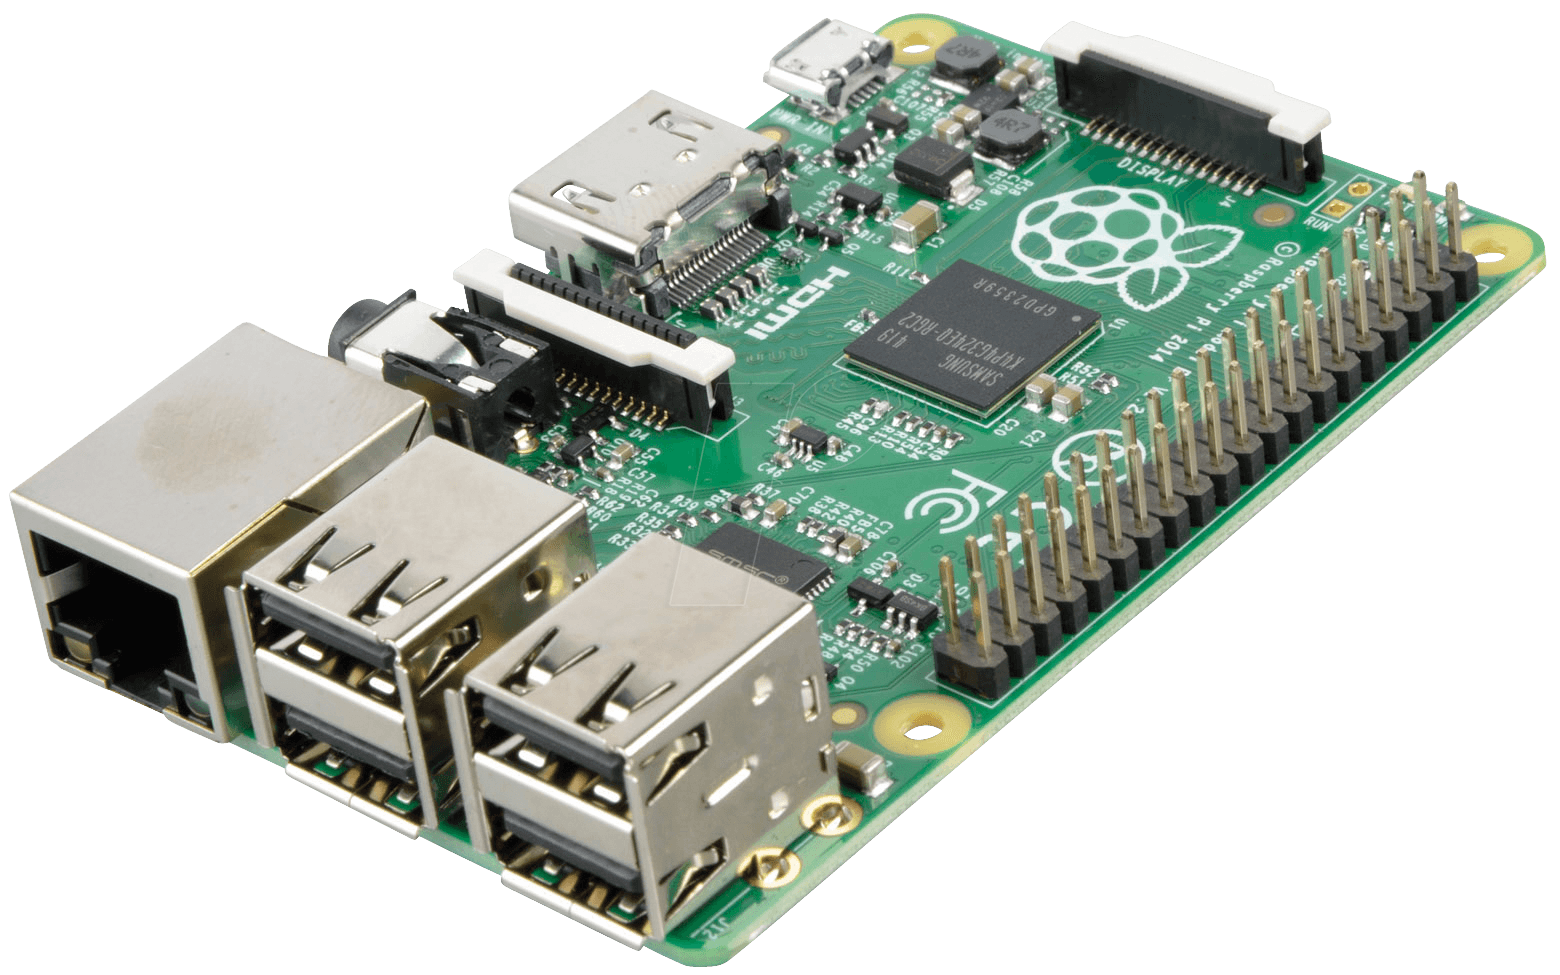
\includegraphics[scale=0.2]{img/cap4/raspberry}
\end{figure}


Il conta persone, come i gateway BLE, è stato implementato sempre usando single board computer
Raspberry.
È dotato inoltre di modulo camera e individua, usando librerie plugAndPlay, le persone che transitano 
dalla porta della biblioteca dove è stato installato.

\begin{figure}[H]
    \centering  
    \caption{Modulo camera per Raspberry}
    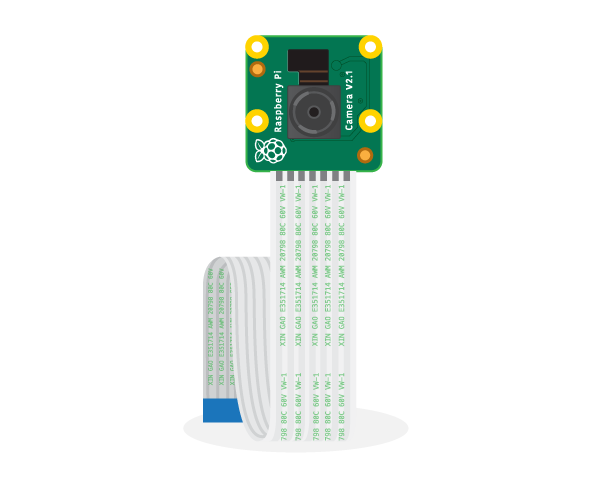
\includegraphics[scale=0.2]{img/cap4/camera}
\end{figure}

Il conta persone mantiene al suo interno un contatore delle persone attualmente dentro l'aula
inviandole con cadenza di 5 minuti ad un microservizio specializzato di eServant che provvede ad
aggiornare il dato sul database.

\chapter{Conclusioni}

Prima di iniziare il mio percorso in Quid Informatica SPA, dove ho contribuito allo
sviluppo del progetto eServant, ho lavorato due anni nella Web Agency fiorentina Aperion SRL.
Nel periodo della web agency mi sono dedicato per passione ai servizi cloud di Amazon
Web Services che mi hanno portato alla finale della competizione mondiale "City on a
cloud", sempre di Amazon Web Services, con il progetto personale \textit{PDENSITY}.

Unendo questa mia esperienza con le alte competenze di Quid Informatica SPA sono 
riuscito ad immergermi a 360° nel progetto di ricerca eServant.\\

La sicurezza sociale oggi giorno è un tema molto acceso su cui dobbiamo
impegnarci a creare strumenti efficaci per salvaguardarla.

L'uso dei braccialetti bluetooth low energy in eServant sono un esempio di questi.
Le allerte automatiche quando la densità delle persone in un determinato varco
supera la soglia limite ne sono un altro.

Sicuramente c'è ancora molta strada da fare per mettere in sicurezza la vita 
sociale, in questo caso legata alla partecipazione di eventi pubblici. eServant 
è una prima soluzione concreta realizzata dal capofila di progetto Quid Informatica SPA.

Ricollegandomi un pò a quella che è stata la mia antecedente esperienza con "City on
a cloud" di Amazon Web Services, oggi giorno abbiamo la grande fortuna di avere
una serie di strumenti ad alto valore tecnologico, aggiungerei PlugAndPlay, pronti
all'uso.
Questo per dire che non dobbiamo più preoccuparci di inventare a basso livello 
nuove intelligenze, come per riconoscimento facciale o altro più avanzato, ma 
concentrarci sul migliorare il processo assemblando e configurando tecnologie
ormai consolidate.

\textbf{Sitografia}
\begin{itemize}
\item [1] sito web eServant \url{http://www.eservant.it}
\item [2] \url{http://coniservizi.it/images/documenti/Rapp_CNEL_maggio_2004.pdf}
\item [3] slide ingegneria del software \url{https://stlab.dinfo.unifi.it/ \\
vicario/Teaching/SW_Engineering/UseCaseDiagsAndTemplates18.pdf}
\item [4] OSGi Alliance \url{http://www.osgi.org}
\item [5] What are microservices? \url{https://microservices.io/}
\item [6] Specifiche Swagger \url{https://swagger.io}
\item [7] Specifiche PostgreSQL \url{https://en.wikipedia.org/wiki/PostgreSQL}
\item [8] Specifiche MongoDB \url{https://en.wikipedia.org/wiki/MongoDB}
\item [9] Specifiche Hibernate ORM \url{https://hibernate.org/orm/}
\item [10] \url{https://codewave.com/insights/mithun-on-switch-to-angular-2 \\
-for-modern-fast-mobile-first-web-apps/}
\item [11] Immagine da \url{https://code.tutsplus.com/tutorials/ionic-from \\
-scratch-what-is-ionic--cms-29323}
\item [12] Tutorial \url{https://ionicframework.com/docs/installation/cli}
\item [13] Immagine da \url{https://ionicframework.com/enterprise/resources/articles/ \\
what-is-apache-cordova}
\item [14] Ionic native camera \url{https://ionicframework.com/docs/native/camera}
\item [15] Specifiche SASS \url{https://sass-lang.com/guide}
\item [16] Specifiche NgRx \url{https://ngrx.io/docs}
\item [17] Immagine da \url{https://blog.imaginea.com/ngrx-introduction-and \\
-its-basic-setup-with-angular/}
\item [18] Protocollo OAauth2.0 https://tools.ietf.org/html/rfc6749
\item [19] History QRcode \url{https://www.qrcode.com/en/history/}
\item [20] Ionic lettura barcode \url{https://ionicframework.com/docs/native/barcode-scanner}
\item [21] A-GPS specifiche \url{https://en.wikipedia.org/wiki/Assisted_GPS}
\item [22] Ionic accesso GPS \url{https://ionicframework.com/docs/native/ \\
geolocation}
\item [23] iBeacon \url{http://www.beaconsandwich.com/what-is-ibeacon.html}
\item [24] Immagine da \url{https://www.businessinsider.com/beacons-and-ibeacons \\
-create-a-new-market-2013-12?IR=T}
\item [25] Prossimità iBeacon \url{https://developer.apple.com/documentation/corelocation/determining_the_proximity_to_an_ibeacon_device}
\item [26] Ionic rilevazione iBeacon \url{https://ionicframework.com/docs/native/ibeacon}
\item [27] Specifiche Rasa \url{https://github.com/RasaHQ/rasa_core}
\item [28] Specifiche AWS lex \url{https://aws.amazon.com/it/lex/}
\item [29] Specifiche Microsoft Luis \url{https://www.luis.ai/home}
\item [30] Specifiche Google Dialogflow \url{https://dialogflow.com/}
\item [31] Material design \url{https://material.io/design/}
\item [32] Material design in Angular \url{https://material.angular.io/}
\item [33] Citazione \url{https://hilton.org.uk/blog/why-naming-things-is-hard}
\item [34] Specifiche BEM \url{http://getbem.com/naming/}
\item [35] Immagine BEM \url{https://medium.com/@dannyhuang_75970/what-is-bem \\
-and-why-you-should-use-it-in-your-project-ab37c6d10b79}
\item [36] Gateway BlueUp  \url{https://www.blueupbeacons.com/index.php?page=gateway}
\item [37] Immagine Raspberry \url{https://www.raspberrypi.org/}
\item [38] Immagine Camera Raspberry \url{https://www.raspberrypi.org/products/camera-module-v2/}
\end{itemize}




%--------------------------------------------------------------
\end{document}
%--------------------------------------------------------------